\chapter{Implementation}
Since communication on Cerebras hardware is limited to the four direct neighbor elements, stencil algorithms that for a single iteration require data from \acp{pe} that are not direct neighbors are far more complex to implement and come with significant communication overhead. For that reason, we limit the scope of this work to update functions that require only communication with the direct neighboring \acp{pe}. This means that the radius of the stencil must be small or equal to the tile size, specifically
\begin{equation}    
\label{eq:radius_constraint}
r \leq \min(t_w, t_h)
\end{equation}

For the simple case where $t_w=t_h=1$, this results in a radius of 1.

Two approaches were implemented:
\begin{itemize}
    \item In specialized version, that restricts the radius to one represents each element of the grid with one \ac{pe} of the \ac{wse}. This specialization allows a heavily optimized implementation, but restricts the maximum problem size to the \ac{wse} hardware dimensions.
    \item A general implementation maps multiple elements of the underlying grid, i.e., a tile size of $t_w, t_h$, to a single \ac{pe} and therefore allows for grid sizes that significantly exceed the \ac{wse} hardware dimensions and a radius greater than one as long as \autoref{eq:radius_constraint} is satisfied. 
\end{itemize}

\section{radius-1, non-tiled}
The computation for each element can be described as follows:
\begin{equation}
    \label{eq:stencil_computation}
    v^{'} = w_0 \cdot v + w_1 \cdot (v_{north} + v_{east} + v_{south} + v_{west})
\end{equation}
Where $v$ is the old value of the element, $v_{north}, v_{east}, v_{south}, v_{west}$ are the values of the four neighbors, $w_0, w_1$ are the stencil coefficients and $v^'$ is the new value of the element.

\subsection{Routing configuration}
Each \ac{pe} must be able to send its data to, and receive data from its four direct neighboring \acp{pe}. Notably it sends the same data to the four neighbors. This allows for increasing communication speed by sending the data only once and forwarding it in the router to all neighbors. We used a pattern containing six distinct colors to map the grid.
The coloring rule can be described as following function $f:\mathbb{N}\times\mathbb{N}\to\{0,1,2,3,4,5\}$:
\begin{equation}
    \label{eq:coloring_function}
    f(x,y) = (x + 2y) \bmod 6
\end{equation}
and visualized in \autoref{fig:r1_stencil_coloring}.
\begin{figure}
    \centering
    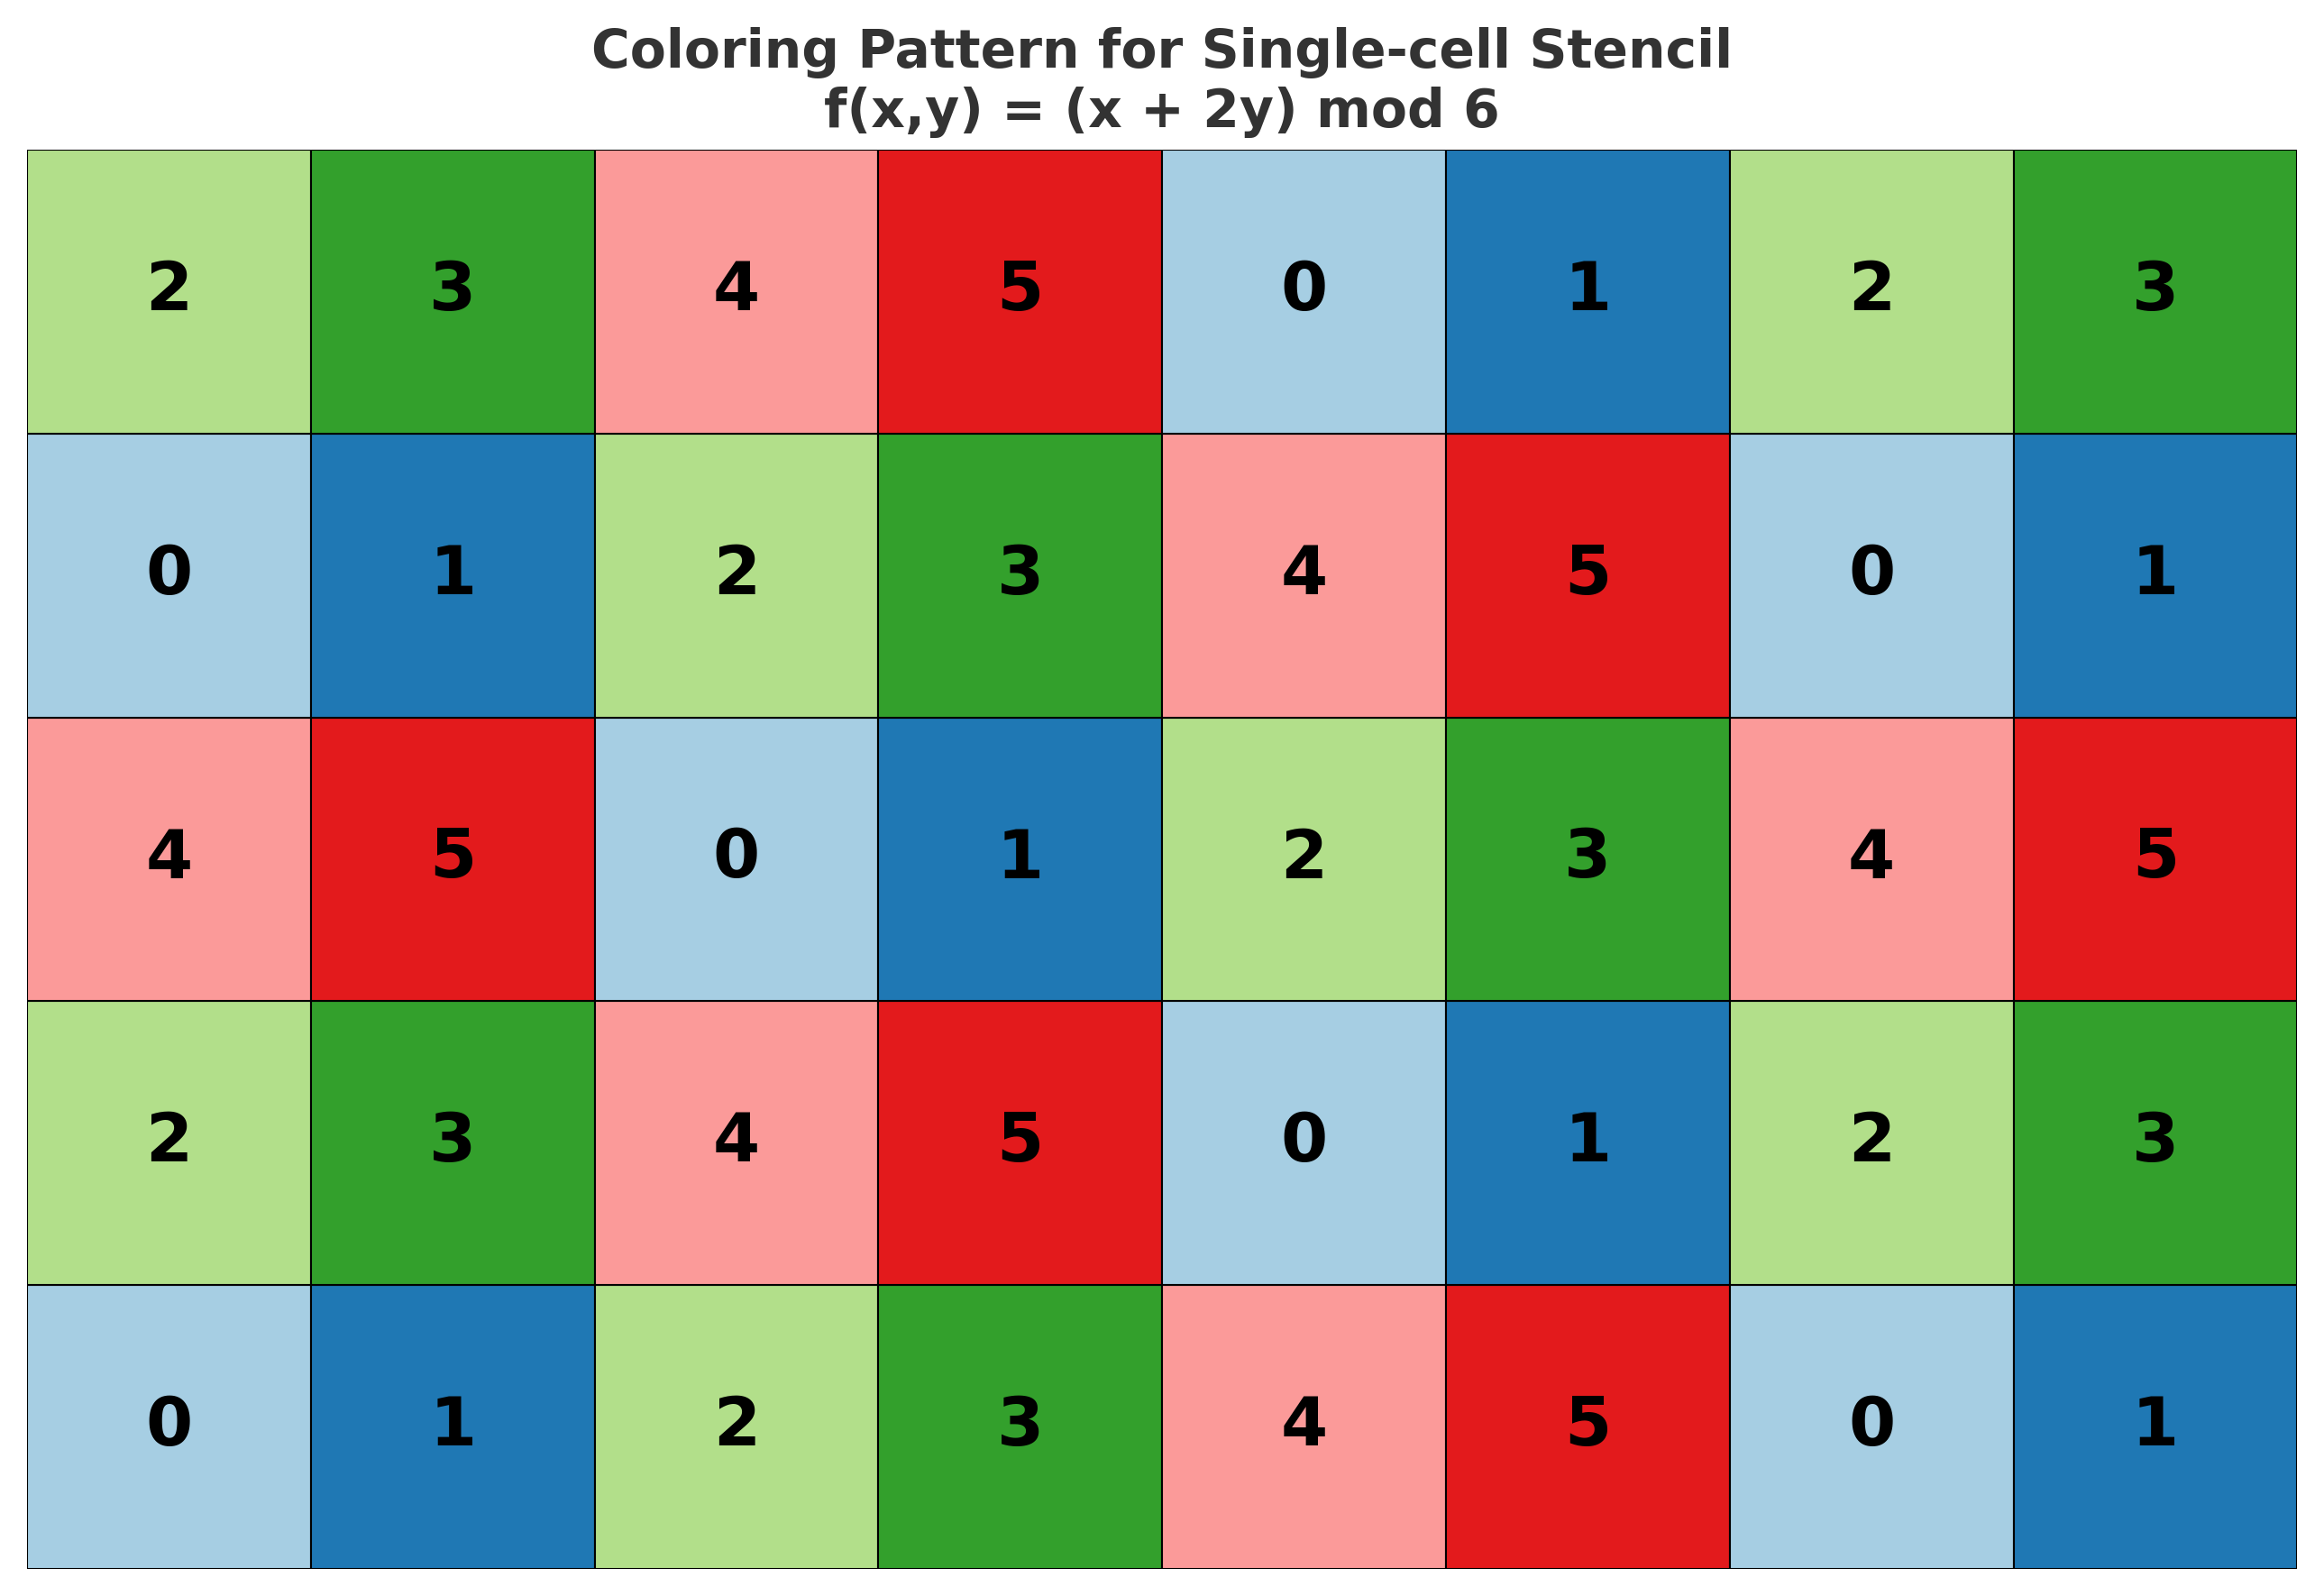
\includegraphics[width=0.5\linewidth]{r1-stencil-coloring.png}
    \caption{Visualization of the coloring pattern for radius-1 non-tiled stencil. Each color represents a distinct routing color (0-5) used for conflict-free communication between \acp{pe}. The numbers in each cell show the color index computed by $f(x,y) = (x + 2y) \bmod 6$.}
    \label{fig:r1_stencil_coloring}
\end{figure}

\subsection{\ac{pe} Program}
The implementation for the radius-1, non-tiled case is relatively simple.
Although only single elements are processed at a time, \acp{dsd} are needed for communication and for performance reasons explicit \ac{dsr} assignment is employed, decreasing the number of cycles per iteration significantly.  
Further, the center multiplication is placed at the beginning of each iteration in a way that it overlaps with the communication delay and does not need an additional cycle.
Because only one fp32 element is received from and send to each neighbour, input- and output- queues never fill up completely and synchronous \ac{dsd} operations can be used instead of asynchronous operations that add significant overhead.
Furthermore, the algorithm multiplies the value which is send to the neighbors with the coefficient $w_1$ while sending, so that the receiving \acp{pe} only add these values to $w_0 \cdot v$ to get the new value.
By computing the intermediate values $intermediate_1$ and $intermediate_2$ before adding them to $value$, the number of cycles for this part of the calculation is reduced from 10 to 7.

\begin{algorithm}[tbh]
    \SetAlgoLined
    \KwData{Received values from neighbors}
    \KwResult{Updated value}
    $intermediate_1 \gets \Call{ReceiveFromNorth}{} + \Call{ReceiveFromEast}{}$\;
    $intermediate_2 \gets \Call{ReceiveFromSouth}{} + \Call{ReceiveFromWest}{}$\;
    $value \gets value + intermediate_1$\;
    $value \gets value + intermediate_2$\;
    \caption{Algorithm with intermediate values}\label{alg:intermediate_values}
\end{algorithm}

While the reason for this performance benefit cannot be explained by the publicly available documentation from Cerebras, speculation from limited testing suggests that values seem to be available to a following operation only three cycles after they were written to.
Our empirical analysis revealed a data dependency stall: an operation using a register as an operand is delayed until at least three cycles have passed since that register was last written to. While this behavior is not detailed in the public documentation, it consistently impacts performance. By reordering the computation to use intermediate variables (as shown in \autoref{alg:intermediate_values}), we mitigate these stalls, reducing the cycle count for this computational segment from 10 to 7 cycles.

Unfortunately, this does not work on WSE-3, since it allows at most one fabric \ac{dsd} arguments per operation.

\begin{table}[h]
    \centering
    \caption{Operations for one grid point and iteration in the radius-1, non-tiled implementation.}
    \label{tab:r1_non_tiled_operations}
    \begin{tabular}{@{}cccc@{}}
        \toprule
        Operation & Cerebras Op Code & Count & Flops \\
        \midrule
        add & \texttt{@fadds} & \num{4} & \num{4} \\
        mul & \texttt{@fmuls} & \num{2} & \num{2} \\
        \midrule
        total & & \num{6} & \num{6} \\
        \bottomrule
    \end{tabular}
\end{table}

\section{tiled any radius star shaped 2d}
For a radius greater than one, the computation can be expressed as follows:
\begin{equation}
    \label{eq:stencil_computation_tiled}
    v^{'} = w_0 \cdot v + \sum_{i=1}^{r} w_i \cdot (v_{north,i} + v_{east,i} + v_{south,i} + v_{west,i})
\end{equation}
Where $v$ is the old value of the element, $v_{north,i}, v_{east,i}, v_{south,i}, v_{west,i}$ are the values of the four neighbors at distance $i$ from the center and $w_0, w_1, \dots, w_r$ are the stencil coefficients.

\subsection{Routing configuration}
\begin{figure}
    \centering
    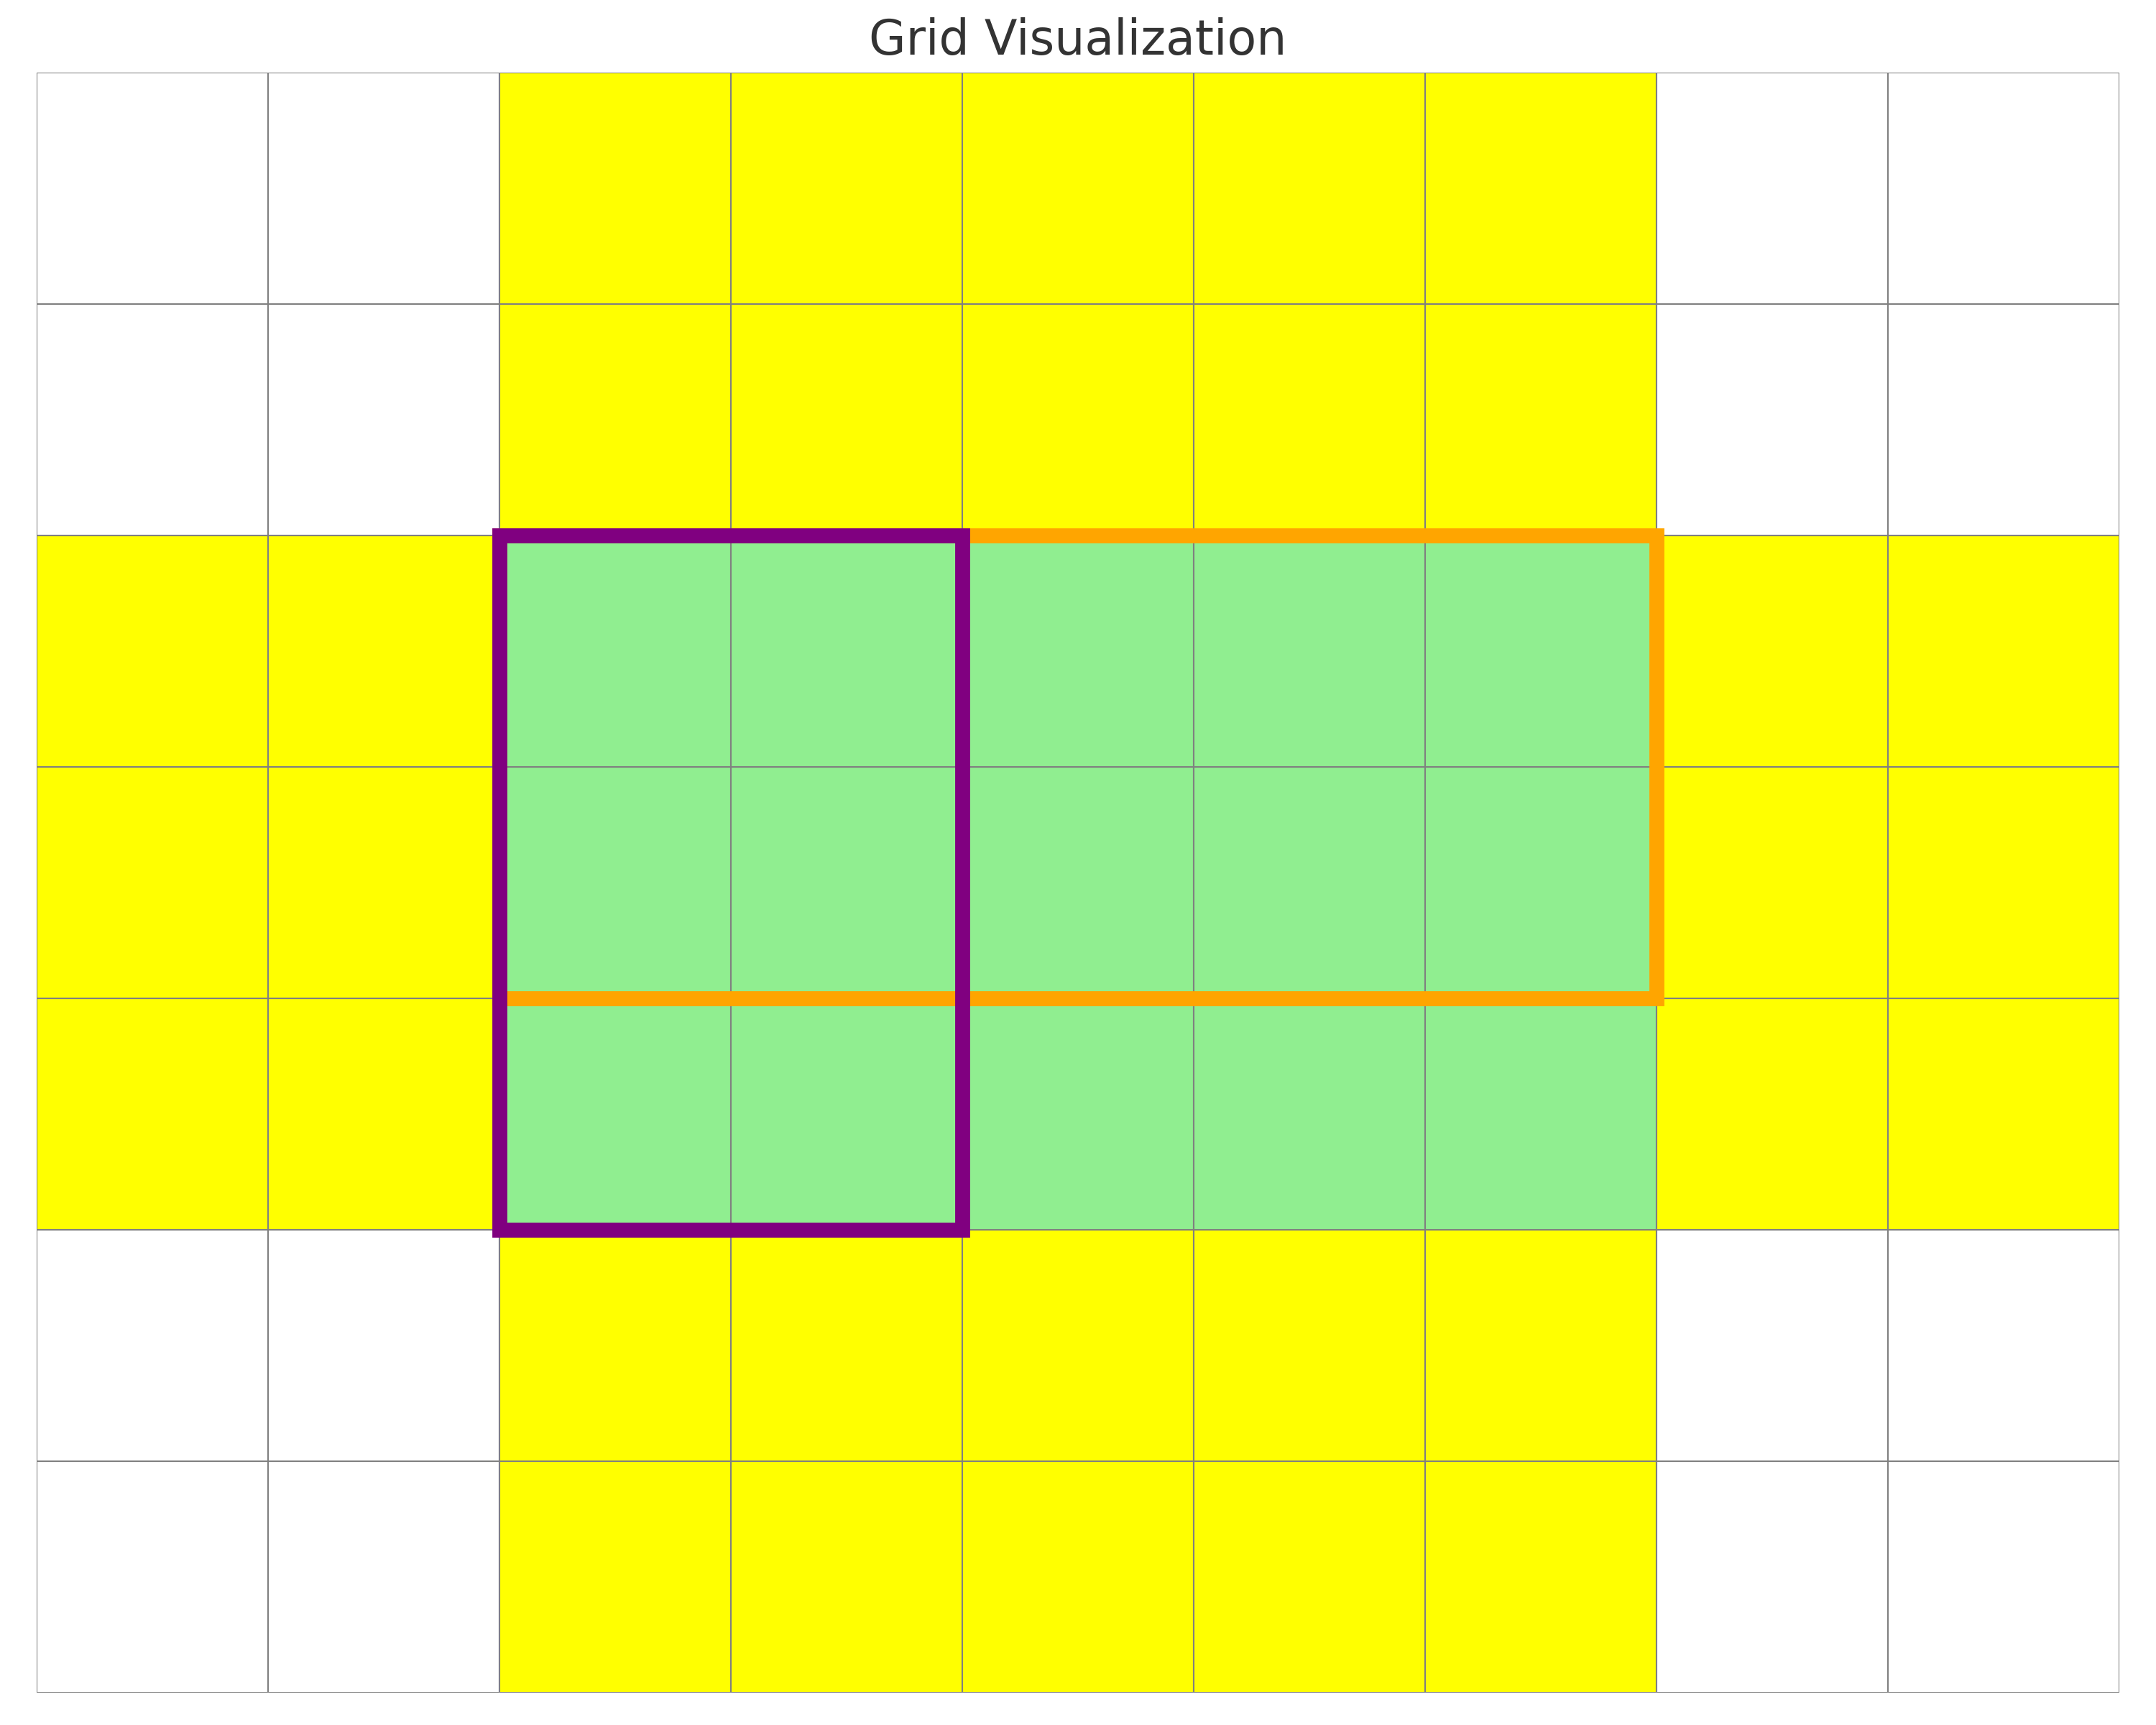
\includegraphics[width=0.5\linewidth]{grid_visualization.png}
    \caption{Visualization of data stored within one \ac{pe} for tiled stencil. $t_w=5$, $t_h=3$ and $r=2$. The green area is the tile of the grid stored within this \ac{pe}. The yellow area is what needs to be received from the neighboring \acp{pe} in order to compute one iteration. The part surrounded in orange is what needs to be send to the northern \ac{pe} and and the purple area is what needs to be send to the western \ac{pe}.}
    \label{fig:grid_visualization}
\end{figure}
The communication for the variable tile size requires one \ac{pe} to send different data to its neighbors. This is visualized in \autoref{fig:grid_visualization}. This requires four distinct colors for sending to the different neighbors as well as four colors to receive. For each of the four directions, a pair of colors is used and arranged in a checkerboard pattern across the \ac{pe}-grid.
If colors 0 and 1 are used for data transfer from west to east, following function can be used to determine what color is used to send and to receive:
\begin{equation}
    \label{eq:tiled_coloring_function}
    f(row, col)=(row+col) \bmod 2
\end{equation}
Where $f$ determines the color used to send data east and $1-f$ is used to receive from west. The same method is also applied for the other directions.

\subsection{\ac{pe} Program}

\begin{figure}
    \centering
    \animategraphics[autoplay,loop,controls=false,width=\linewidth]{0.5}{stencil_frames/frame_0}{0}{8}
    \caption{Visualization of the stencil computation for a radius-2, tiled stencil. (animation might not play in all pdf readers)}
    \label{fig:stencil_algorithm_animation}
\end{figure}

The tile of the grid, held by single \ac{pe} is stored in the center region of a 2D array of size $(t_h+2r)\times (t_w+2r)$ - the $buffer$. This array is larger than the tile itself to allow for the halo region, which is used to store the data received from the neighbors. Furthermore an accumulator array of the same size is used to store the intermediate values of the stencil computation. In this array, only the center of size $t_h, t_w$ is used. Choosing its size to be the same as the buffer leads to more consistent memory access patterns, which reduces bank conflicts.

Two \texttt{mem4d\_dsd}s per direction are used for communication. One that specifies the location within the buffer of the data to send and one that specifies the location of the data to receive.
Asynchronous \texttt{@fmovs} instructions are used for data exchange. Two counters track the completion of asynchronous send and receive operations. Once all four neighbor data blocks have been sent and all four have been received, the main computation task is triggered. This ensures that the computation only starts once all necessary data is available in the halo regions.

A \ac{dsd} is used to select the center region of the buffer. This \ac{dsd} is subsequently shifted to represent a rectangular area of the buffer that is shifted up, down, left or right by a number of elements up to the radius from the center. \texttt{@fmacs} instructions are used to multiply these values with the respective weight and add the results to the accumulator. The accumulator is then multiplied with the weight $w_0$ and added to the center region of the buffer to complete the iteration. This process is visualized in \autoref{fig:stencil_algorithm_animation}.

If only \texttt{@fmacs} instructions were used, the accumulator would have to be reset to zero after each iteration. To avoid this, a \texttt{@fmuls} instruction is used for the very first operation that writes to the accumulator to overwrite the values of the previous iteration.

\begin{algorithm}[tbh]
    \SetAlgoLined
    \KwData{Buffer with halo regions filled}
    \KwResult{Updated buffer center}
    \For{$i \gets 1$ \KwTo $r$}{
        \eIf{$i == 1$}{
            $accumulator \gets weights[i] \cdot buffer\_center\_dsd_{UP,i}$\;
        }{
            $accumulator \gets accumulator + weights[i] \cdot buffer\_center\_dsd_{UP,i}$\;
        }
        $accumulator \gets accumulator + weights[i] \cdot buffer\_center\_dsd_{DOWN,i}$\;
        $accumulator \gets accumulator + weights[i] \cdot buffer\_center\_dsd_{LEFT,i}$\;
        $accumulator \gets accumulator + weights[i] \cdot buffer\_center\_dsd_{RIGHT,i}$\;
    }
    $buffer\_center\_dsd \gets buffer\_center\_dsd + weights[0] \cdot accumulator$\;
    \caption{Tiled algorithm code}\label{alg:tiled_algorithm}
\end{algorithm}

The dicrilet border is implemented by using a ring of \acp{pe} that only send and receive data from their neighbors and do not participate in the computation. If $r<t_w$ or $r<t_h$ the border \acp{pe} values are padded with zeros to fill their buffer. Re refer to the \acp{pe} that only send and receive data from their neighbors as border \acp{pe}, the ones that participate in the computation as inner \acp{pe} and the set of both of these as active \acp{pe}.

\begin{table}[h]
    \centering
    \caption{Operations for one grid point and iteration, tiled implementation with radius $r$.}
    \label{tab:tiled_operations}
    \begin{tabular}{@{}cccc@{}}
        \toprule
        Operation & Cerebras Op Code & Count & Flops \\
        \midrule
        fmac & \texttt{@fmacs} & $5r-1$ & $10r-2$ \\
        mul & \texttt{@fmuls} & \num{1} & \num{1} \\
        \midrule
        total & & $5r$ & $10r-1$ \\
        \bottomrule
    \end{tabular}
\end{table}

As a special case of the tiled algorithm, the radius-1 problem was further optimized by using \texttt{mem1d\_dsd}s instead of \texttt{mem4d\_dsd}s for the halo regions where the neighbors data is received as well as the data to send. Furthermore the shifted \acp{dsd} are precomputed and all \acp{dsd} are explicitly assigned to distinct \acp{dsr}. There are enough \acp{dsr} available so that each \ac{dsr} is used for at most one \ac{dsd}. This allows for a significant reduction in the number of cycles per iteration, since loading the \acp{dsd} into \acp{dsr} only needs to be done once, independent of the number of iterations. We still find that the \acp{dsd} used for reading the parts of the buffer that are send to the neighbors and the ones describing the halo regions for receiving need to be reloaded to the \acp{dsr} for each iteration. The load to \ac{dsr} for these \acp{dsd} acts as a kind of reset and if not done, it leads to buffer overflows. The documentation doesn't specify this requirement and interestingly, it is not necessary for all \acp{dsd}. 
As another optimization, \texttt{@fadds} are used instead of \texttt{@fmacs} and the multiplication is handled separately. This reduces the flop number from $9$ to $6$ per element and results in a performance improvement because the simd width for \texttt{@fadds} is 2/4 on wse-2/3 while it is only 1 for \texttt{@fmacs}. Note that the shifted \acp{dsd} $buffer\_center\_dsd_{DIR,i}$ in the general version need to be created for each iteration of the loop while pre-computed \acp{dsd} are used in this optimized version.

We refer to this as the r1 optimized version of the tiled algorithm.
The tiled algorithm is implemented so that it automatically selects the r1 optimized version if the radius is 1.
For all experiments in this work, the r1 optimized version is used whenever applicable, except when explicitly stated otherwise.

\begin{algorithm}[tbh]
    \SetAlgoLined
    \KwData{Buffer with halo regions filled}
    \KwResult{Updated buffer center}
    $accumulator \gets buffer\_center\_dsd \cdot weights[0]/weights[1]$\;
    $accumulator \gets accumulator + buffer\_center\_dsd_{UP,1}$\;
    $accumulator \gets accumulator + buffer\_center\_dsd_{DOWN,1}$\;
    $accumulator \gets accumulator + buffer\_center\_dsd_{LEFT,1}$\;
    $accumulator \gets accumulator + buffer\_center\_dsd_{RIGHT,1}$\;
    $buffer\_center\_dsd \gets buffer\_center\_dsd + accumulator \cdot weights[1]$\;
    \caption{Radius-1, tiled algorithm code}\label{alg:r1_tiled_algorithm}
\end{algorithm}

\begin{table}[h]
    \centering
    \caption{Operations for one grid point and iteration, r1 optimized tiled implementation.}
    \label{tab:tiled_operations_r1_optimized}
    \begin{tabular}{@{}cccc@{}}
        \toprule
        Operation & Cerebras Op Code & Count & Flops \\
        \midrule
        add & \texttt{@fadds} & \num{4} & \num{4} \\
        mul & \texttt{@fmuls} & \num{2} & \num{2} \\
        \midrule
        total & & \num{6} & \num{6} \\
        \bottomrule
    \end{tabular}
\end{table}

With a larger tile size, the explicit starting mechanism of the computation task can be skipped so that the computation task can be activated while the data is send and received. Explicitly specified task priorities lead to the computation task only being executed after all data is send and received. However, this only works for WSE-3. 